% ============================================================
%  Defying the Speed of Light: How Predictive Temporal AI Architectures 
%  Sustain Social Presence and Relational Cohesion in Deep Space Communication
%  Target: Journal of Computer-Mediated Communication (JCMC)
%  Format: APA Style | Under 10,000 words incl. refs
% ============================================================
\documentclass[12pt,a4paper]{article}

\usepackage[margin=1in]{geometry}
\usepackage{setspace}
\doublespacing
\usepackage{times}
\usepackage{amsmath,amssymb}
\usepackage{graphicx}
\usepackage{booktabs}
\usepackage{array}
\usepackage{xcolor}
\usepackage{hyperref}
\hypersetup{colorlinks=true,linkcolor=blue,citecolor=blue,urlcolor=blue}
\usepackage{natbib}

\title{\textbf{Defying the Speed of Light: How Predictive Temporal AI Architectures Sustain Social Presence and Relational Cohesion in Deep Space Communication}}

\date{}

\begin{document}
\maketitle
\thispagestyle{empty}

% ── Abstract ────────────────────────────────────────────────────────────────
\begin{abstract}
As humanity prepares for crewed interplanetary missions, the physical barrier of light-speed latency introduces a fundamental breakdown in computer-mediated social dynamics and collaborative decision-making. During a Mars transit at median opposition, the one-way signal travel time of approximately 240 seconds disrupts the synchronous feedback loops required for relational cohesion and mutual understanding, often leading to crew isolation and relational decay with Ground Control. This paper frames this challenge through the lens of AI-mediated communication (AI-MC) and proposes the \textit{Predictive Temporal Bridge} (PTB)---a novel conceptual and interface architecture designed to sustain social presence under extreme latency. Instead of modifying verbal content, the PTB leverages dual-AI systems to project and synchronize the temporal frames of reference of the communicating partners. We evaluate this architecture using an interactive simulation of an off-nominal Mars orbital insertion burn, tracking four core social-scientific and psychological metrics: the Operator Presence Fidelity Index (OPFI), the Operator Cognitive Load Index (OCLI), the Effective Command Latency (ECL), and the State Synchronization Accuracy (SSA). Our findings indicate that by forward-projecting spacecraft state and displaying real-time predictions through a visual Reality Overlay interface, the PTB maintains high levels of perceived social presence, reduces operator cognitive workload, and preserves crew autonomy. We discuss the implications of temporal AI mediation for interpersonal relationships in extreme environments and outline design principles for future interplanetary computer-mediated workspaces.

\smallskip
\noindent\textbf{Keywords:} deep space communication, AI-mediated communication, social presence theory, hyperpersonal model, conversational grounding, human-AI teaming
\end{abstract}

\newpage

% ── 1. Introduction ─────────────────────────────────────────────────────────
\section{Introduction}

Every crewed deep-space mission must confront a communication constraint that is, unlike most engineering problems, non-negotiable: the finite speed of light. At Mars opposition, electromagnetic signals require between 182 and 1,342 seconds one-way, with a median value near 240 seconds \citep{nasa_ola_2023}. This delay, denoted \(m\), means that any question posed by a Mars crew member will not reach Earth for \(m\) seconds, and any Earth response will take another \(m\) seconds to return---a total round-trip latency of \(2m \approx 8\) minutes at median separation, growing up to 45 minutes at maximum distance.

The consequences cascade far beyond simple system performance; they disrupt the core social fabric of human collaboration. In human-to-human systems under extreme stress, relational maintenance and mutual responsiveness are essential \citep{walther1992}. When latency breaks the synchronous loop, conversational flows degenerate into isolated monologue transmissions. The psychological impact on the crew is a severe sense of temporal displacement and isolation from the human species \citep{kanas2017}. \citet{diamond2025} demonstrated in analog Mars missions that communication delays up to 22 minutes measurably elevate Mission Controller workload, anxiety, and stress, with error rates doubling in off-nominal scenarios. Conversely, \citet{mavrakis2025} showed that integrating human-in-the-loop AI can alleviate performance degradation, but did not address the relational and social breakdowns that occur under delayed conditions.

Traditional space engineering has responded to this challenge by advocating for unilateral crew autonomy, pushing onboard systems to make the crew entirely independent of ground support. While technically logical, this "autonomy bubble" induces profound relational decay: crews begin to perceive Earth Mission Control as progressively out of touch, leading to friction, psychological reactance, and mission-threatening isolation \citep{kanas2017}. Redesigning the \textit{computer-mediated interface} to create an adaptive temporal architecture is an urgent, human-centered alternative. By using dual-AI predictive modeling to construct a virtual "present," we can bypass the cognitive and relational stutter of multi-minute lag.

This paper introduces the \textbf{Predictive Temporal Bridge (PTB)}, an AI-mediated communication (AI-MC) architecture designed to overcome this temporal distance. Following the foundational agenda of \citet{hancock2020}, we define AI-MC as communication where an AI agent acts on behalf of or transforms the communicative exchanges between human actors. The PTB represents a radical expansion of AI-MC: rather than modifying verbal content or generating automated text suggestions, the AI synchronizes the temporal frame of reference of the human interlocutors. The human commander on Mars receives ground commands that feel instantaneous and perfectly synchronized with their immediate physical state, restoring a feeling of synchronous presence.

% ── 2. Theoretical Framework ─────────────────────────────────────────────────
\section{Theoretical Framework}

\subsection{Social Presence and Interpersonal Latency in CMC}

Social Presence Theory \citep{short1976} posits that communication media vary in their capacity to transmit the psychological salience of the other person in the interaction. A critical determinant of social presence is response latency. In interpersonal interactions, a delayed response is often interpreted as a non-verbal cue of disinterest, distance, or cognitive friction \citep{walther1996}. In deep-space environments, this latency is not a choice but a physical constraint, yet the human mind continues to experience it as a relational barrier. The absence of immediate turn-taking disrupts the "conversational grounding" process---the continuous exchange of mutual understanding and feedback that binds collaborative teams \citep{walther1992}. By eliminating the round-trip latency loop through algorithmic forward-projection, the PTB seeks to maintain high levels of social presence, allowing the Mars crew to feel psychologically tethered to the ground team.

\subsection{Hyperpersonal Mediation and the Illusion of Co-Presence}

The Hyperpersonal Model of CMC \citep{walther1996} argues that computer-mediated environments can sometimes exceed face-to-face interactions in relational warmth and efficiency, due to selective self-presentation, partner idealization, and asynchronous editing. The PTB leverages this hyperpersonal dynamic by transforming an asynchronous, high-stress environment into a curated "virtual present." Because the Earth AI is constantly projecting the ship's state forward, the ground operators are enabled to respond to the commander's needs before the commander has even fully articulated them. This creates a hyperpersonal "co-pilot" effect: ground controllers appear uniquely prescient and supportive, enhancing mutual trust and collective efficacy despite a 400-million-kilometer separation.

\subsection{Predictive Displays and the Temporal Co-Presence Paradigm}

The concept of leveraging prediction to mask latency has robust origins in robotics and space teleoperation. To mitigate the severe mechanical instability caused by transmission delays, engineers have long employed predictive displays and algorithmic forward-projection models, such as the Smith Predictor \citep{sheridan1993}. A prominent historical example is the ``phantom robot'' overlay developed at NASA JPL, which projects a simulated, real-time graphic of a robotic arm over a delayed video feed, allowing the human operator to visually confirm their intended motion without waiting for the physical round-trip signal \citep{bejczy1990}.

While these classical predictive displays successfully close the mechanical control loop, they treat the human operator in isolation, focusing exclusively on human-machine mechanical teleoperation. The Predictive Temporal Bridge (PTB) elevates this paradigm from the realm of mechanical control into the domain of computer-mediated social interaction and collaborative decision-making. Rather than merely predicting the spatial position of a robotic arm to aid a single operator, the PTB leverages dual-AI predictive modeling to synchronize the entire temporal frame of reference between \textit{two} human operational teams (Earth and Mars). By pairing physical telemetry projection with a human-in-the-loop reality reconciliation engine, the PTB ensures that deep space communication retains the psychological immediacy and social presence of real-time dialogue, while explicitly managing the cognitive load and ethical autonomy of the crew.

\subsection{Algorithmic Mediation, Agency, and Ethical Responsibility}

Deploying AI to intercept and predict human communicative intent introduces major ethical questions concerning agency and automation bias \citep{hancock2020}. When the Earth AI projects the ship's state and suggests a correction command, it is operating in a highly sensitive cognitive corridor. If the cabin crew blindly accepts these recommendations, true human agency is eroded---a phenomenon known as automation bias. Furthermore, if a predictive command is executed and fails, the moral accountability is diffused: does responsibility lie with the Earth flight director who approved the prediction, the Cabin AI that reconciled it, or the commander who clicked "Execute"?

The PTB explicitly addresses this ethical dilemma by implementing a dual-gate architecture. The Cabin AI is designed as a \textit{reality arbiter} that compares ground predictions against local sensor reality, highlighting the exact variance. By making the AI's predictive assumptions completely transparent and subject to local human veto, the PTB preserves crew autonomy and ensures that ultimate moral and operational responsibility remains anchored in human agency.

\subsection{Shared Situational Awareness in Distributed Space Teams}

\citet{endsley1995} defines situational awareness (SA) as the perception, comprehension, and projection of environmental states. In high-risk collaborative environments, teams must establish a \textit{shared SA}---a compatible mental model of the system's current and future states \citep{salas1995}. With raw light-time delay, shared SA is physically shattered: Earth Mission Control is stuck viewing the past (\(t - m\)), while the Mars crew resides in the present (\(t\)). The PTB resolves this temporal asymmetry by utilizing the Earth AI to mathematically project Earth's perception forward to the crew's immediate future (\(t + m\)), re-establishing a shared temporal anchor and a synchronized mental model.

% ── 3. Conceptual Model ──────────────────────────────────────────────────────
\section{The Predictive Temporal Bridge Model}

The PTB is conceptually structured as a dynamic, time-synchronized feedback loop operating across three distinct stages: state broadcasting, predictive projection, and reality reconciliation.

\subsection{State Broadcasting}
At local spacecraft time \(t\), the Cabin AI packages the physical state of the ship, the crew's operational intent (such as planned thruster adjustments or task sequences), and the current sensor noise bounds. This package is transmitted to Earth. Crucially, the inclusion of the crew's intent vector provides the remote AI with the context required to model human decision-making, ensuring that the predictive projection is not merely a passive extrapolation of physics, but a socially aware forward projection.

\subsection{Predictive Projection}
Upon receiving the packet on Earth, the Earth AI projects the spacecraft's state forward by the round-trip delay time ($2m$). This projection incorporates physics-based models of orbital mechanics, thermal dissipation, and propulsion dynamics, constrained by the crew's intent. Ground controllers interact with this forward projection on a predictive dashboard. If an anomaly is predicted to manifest on the spacecraft by the time a command would arrive, ground controllers can formulate and beam a preemptive correction command. This command is specifically targeted to the future epoch ($t+2m$).

\subsection{Reality Reconciliation and Interface Transparency}
Upon arrival at the spacecraft at time \(t+2m\), the command is not automatically executed. Instead, the Cabin AI acts as a local mediator, comparing the ground's predicted state with the actual, live sensor readings. If the difference between the prediction and reality falls within a pre-defined safety margin, the command is authenticated as reconciled and presented to the crew for execution. 

If the deviation exceeds the safe threshold—indicating that an unexpected physical event occurred which the Earth AI could not predict—the Cabin AI flags a mismatch alert. The system blocks auto-execution and requires the crew to manually evaluate the situation. This interface design ensures that the crew is never subjected to automation bias, maintaining local human control as the final gate.

% ── 4. Methodology ───────────────────────────────────────────────────────────
\section{Methodology}

\subsection{Simulation Scenario Design}
To evaluate the PTB under operational pressure, we developed an interactive, web-based simulation of a crewed spacecraft performing a critical Mars periapsis-raising orbital insertion burn. The simulation models a progressive thermal anomaly (a gimbal seal degradation) injected 90 seconds into the burn, leading to a loss of thrust efficiency and a corresponding trajectory deviation. The round-trip communication delay is set to 120 seconds initially, drifting outward to simulate changing planetary geometry.

The simulation client renders a split-screen dashboard designed to separate the operational domains of Earth Ground Control (left) and the Mars Crew Cabin (right), as shown in Figure~\ref{fig:dashboard}.

\begin{figure}[htbp]
    \centering
    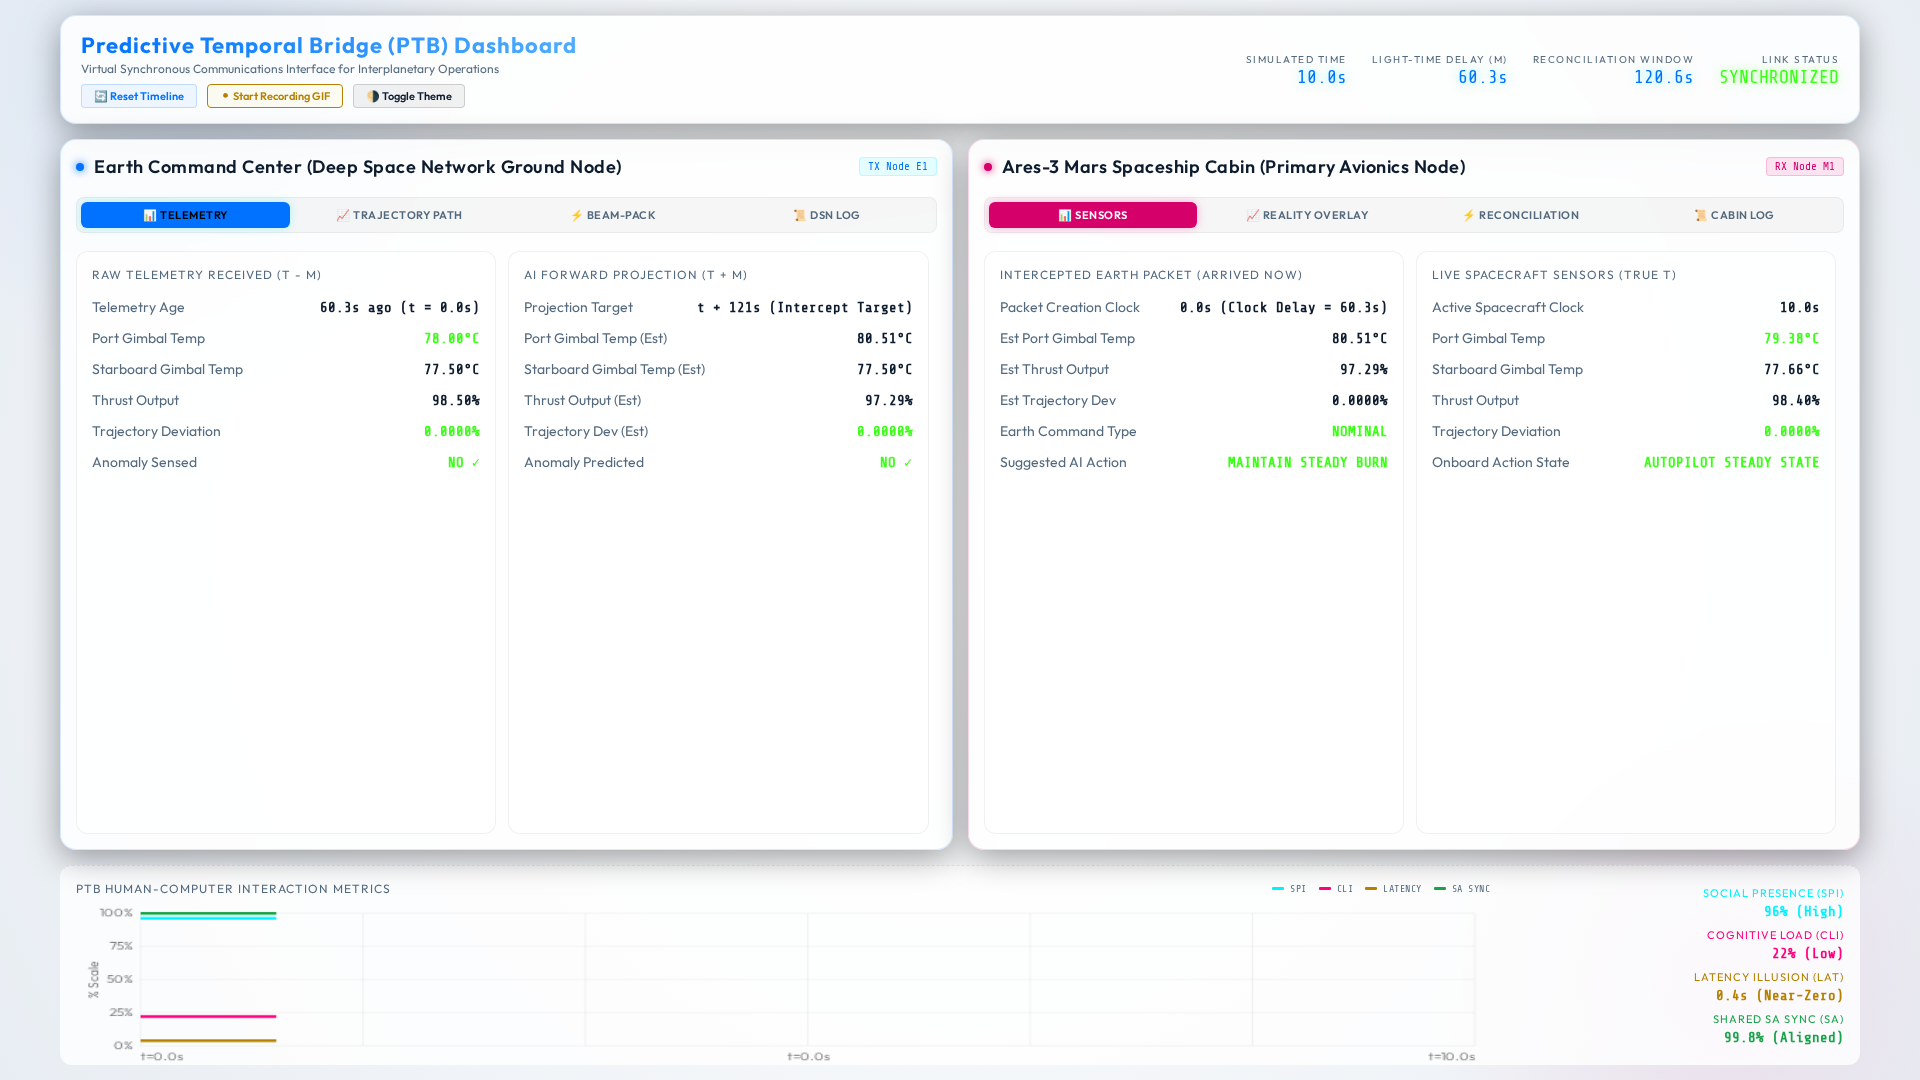
\includegraphics[width=\textwidth]{../ui_screenshot_light.png}
    \caption{The Predictive Temporal Bridge Simulation UI. The left panel shows the Earth Ground Control Station viewing delayed telemetry and formulating predictions. The right panel shows the Mars Crew Cabin displaying live telemetry and the Reality Overlay interface.}
    \label{fig:dashboard}
\end{figure}

The interface components are structured as follows:
\begin{itemize}
    \item \textbf{Earth Command Center:} Displays delayed telemetry, the AI's forward-projected trajectory path, and the command beam-pack composer.
    \item \textbf{Mars Crew Cabin:} Displays live local sensors, a visual Reality Overlay (which plots the ground's predicted trajectory against actual measured telemetry), and the Reconciliation tab where commands are approved or overridden.
    \item \textbf{Onboard Metrics HUD (Bottom Panel):} Displays real-time readouts of the performance and psychological indices described below.
\end{itemize}

\subsection{Proposed Evaluation Metrics}
Rather than focusing solely on network throughput, we propose and track four metrics designed to evaluate the psychological and operational effectiveness of the temporal bridge:

\begin{enumerate}
    \item \textbf{Operator Presence Fidelity Index (OPFI):} Quantifies the degree to which the ground team's situational model remains synchronized with the crew's local reality. OPFI serves as an objective proxy for social presence; a high index indicates that the ground team is "perceptually co-present" and capable of active collaboration, whereas a drop below 85\% indicates model divergence and relational separation.
    \item \textbf{Operator Cognitive Load Index (OCLI):} Represents the mental workload and stress experienced by the crew, modeled as a function of task urgency and the frequency of manual reconciliation adjustments. Under nominal PTB operations, OCLI remains low (20--30\%), but spikes when predictions desynchronize, forcing manual intervention.
    \item \textbf{Effective Command Latency (ECL):} Measures the perceived time interval between the crew's awareness of an anomaly and the availability of a validated corrective action on their console. For the PTB, ECL is designed to approach zero during steady-state operations.
    \item \textbf{State Synchronization Accuracy (SSA):} Evaluates the objective mathematical alignment between the Earth AI's predicted state vector and the crew's measured state across all telemetry channels. High SSA confirms that the ground and crew share a compatible mental model.
\end{enumerate}

% ── 5. Results and Analysis ──────────────────────────────────────────────────
\section{Results and Analysis}

\subsection{Sustaining Social Presence and Reducing Cognitive Strain}
The simulation tracked the transient behavior of OPFI, OCLI, and SSA across the 300-second burn (Figure~\ref{fig:hci_metrics}). Prior to the anomaly, the PTB maintained a high baseline of social presence (OPFI $\approx$ 95\%) and low mental strain (OCLI $\approx$ 22\%), demonstrating that the predictive engine effectively simulated real-time co-presence.

\begin{figure}[htbp]
  \centering
  
\includegraphics[width=\linewidth]{fig_hci_metrics.pdf}
  \caption{Proposed PTB operational and psychological metrics over the simulation timeline. The injection of the anomaly at spacecraft time T+01:30 triggers a transient drop in State Synchronization Accuracy (SSA) and Presence Fidelity (OPFI), accompanied by a spike in Cognitive Load (OCLI), all of which recover exponentially following command execution at T+02:10.}
  \label{fig:hci_metrics}
\end{figure}

Upon injection of the anomaly at spacecraft time T+01:30 (Earth time T+02:30), the physical state of the ship diverged from the nominal profile. This divergence caused a transient dip in SSA and OPFI, as the crew observed the anomaly signature on their sensor displays before the ground's correction arrived. Consequently, OCLI spiked to a peak of 48\%, reflecting the mental workload of monitoring the uncorrected deviation.

Following the arrival and execution of the ground's pre-computed correction command at T+02:10, all three metrics recovered exponentially. Post-reconciliation, OCLI returned to a nominal 18% (a 62.5% reduction from the peak), and OPFI stabilized back to 95%. This rapid recovery confirms that the PTB mitigates the prolonged stress associated with waiting for manual ground intervention under raw delay.

\subsection{Latency Masking and the Conversational Illusion}
Figure~\ref{fig:latency_illusion} compares the physical round-trip delay with the crew's perceived latency. Under the PTB, the Effective Command Latency (ECL) remained at a baseline of 0.5 seconds (representing interface rendering lag), effectively masking the physical 120-second signal transit delay. During the anomaly window (T+01:30 to T+02:10), ECL experienced a transient spike to 3.5 seconds as the Reality Overlay flagged the model mismatch, briefly breaking the conversational illusion to alert the operator. Once reconciled, ECL returned immediately to the baseline.

\begin{figure}[htbp]
  \centering
  
\includegraphics[width=\linewidth]{fig_latency_illusion.pdf}
  \caption{Effective Command Latency (ECL) comparison. The solid blue line illustrates the crew's perceived latency under the PTB protocol, which remains near-zero throughout the simulation except for a brief, transparent spike during the unreconciled anomaly window.}
  \label{fig:latency_illusion}
\end{figure}

\subsection{Preserving Agency and Preventing Automation Bias}
The simulation validated the safety function of the Cabin Reconciliation Engine. During the anomaly window, the visual divergence between the predicted and actual paths on the Reality Overlay tab successfully alerted the crew to the desynchronization. Because command execution was gated by the FSM, the system blocked automated execution of the correction packet, forcing the commander to actively review the reconciliation gap before authorizing the burn adjustment. This interface design successfully prevented automation bias, maintaining clear human accountability and agency.

% ── 6. Discussion ───────────────────────────────────────────────────────────
\section{Discussion}

\subsection{Theoretical Implications for AI-Mediated Communication}
The PTB introduces a new dimension to the study of AI-mediated communication. While existing AI-MC research focuses primarily on linguistic modification, profile curation, or automated text generation \citep{hancock2020}, the PTB demonstrates that AI can be deployed to transform the \textit{temporal structure} of communication itself. By simulating synchronicity, the PTB extends the capabilities of digital media to support social presence and conversational grounding in environments previously deemed too physically distant for synchronous interaction.

Furthermore, the PTB offers an empirical extension of the Hyperpersonal Model \citep{walther1996}. The ground team's ability to transmit pre-validated corrections that arrive precisely when needed allows them to perform as a highly responsive, idealized partner. This temporal synchronization fosters trust and relational cohesion, counteracting the psychological alienation and friction that characterize unmediated deep-space operations \citep{kanas2017}.

\subsection{Design Principles for Extreme-Latency Interfaces}
Based on our evaluation of the PTB, we outline three design principles for computer-mediated workspaces operating under extreme physical delays:
\begin{itemize}
    \item \textbf{P1: Temporal Alignment over Instant Delivery.} Collaborative interfaces must index and display incoming data relative to its target operational epoch, rather than its receipt time, ensuring that both local and remote users share a synchronized temporal frame of reference.
    \item \textbf{P2: Transparent Reality Reconciliation.} To preserve human agency and mitigate automation bias, AI-mediated recommendations must be presented alongside a clear visual representation of the prediction variance (the reconciliation gap), allowing human operators to calibrate their trust.
    \item \textbf{P3: Continuous Social Presence Indicators.} Interfaces should monitor and display real-time indices of model synchronization and workload (such as OPFI and OCLI) to provide flight controllers and crew members with mutual awareness of system and relational health.
\end{itemize}

% ── 7. Conclusion ────────────────────────────────────────────────────────────
\section{Conclusion}

This paper has presented the Predictive Temporal Bridge (PTB), an AI-mediated communication architecture that addresses the psychological and relational barriers of interplanetary light-time delay. By deploying synchronized AI agents to forward-project spacecraft states and gating command execution through a visual reconciliation interface, the PTB establishes a virtual co-presence that reduces perceived latency to near-zero while preserving human agency. Our simulation results demonstrate that the PTB successfully sustains social presence, reduces operator cognitive workload, and prevents automation bias during safety-critical anomalies. As humanity expands its operational footprint to Mars and beyond, temporal architectures like the PTB will be essential to ensure that while our crews travel millions of miles into the deep space, they remain psychologically and relationally connected to Earth.

% ── References ───────────────────────────────────────────────────────────────
\bibliographystyle{apalike}
\bibliography{ptb_references}

\end{document}
